\documentclass{article}
\usepackage{authblk}
\usepackage{mathptmx}
\usepackage{url,latexsym,amsmath,amsthm,xspace,rotating,multirow,multicol,xspace,amssymb,paralist}
\usepackage{euscript}
\usepackage{fancybox,xcolor}
\usepackage{longtable}
\usepackage{paralist}
\usepackage[normalem]{ulem}
\usepackage[pdftex]{hyperref}
\usepackage{algorithmicx}
\usepackage{algpseudocode}
\usepackage{algorithm}
\usepackage{cancel}
\usepackage{mathtools}

\usepackage{url}
\usepackage{latexsym}

\usepackage{times}
\usepackage{amsmath}
\usepackage{amsthm}
\usepackage{amssymb}
\usepackage{graphicx}
\usepackage{xspace}
\usepackage{tabularx}
\usepackage{multicol}
\usepackage{multirow}
%\usepackage{hyperref}
\usepackage{url}
%\usepackage{natbib}
\usepackage{wrapfig}
\usepackage{comment}
\usepackage{listings}
\usepackage{color}
\usepackage[utf8]{inputenc}
\usepackage{fancyvrb}
\usepackage{booktabs}
\usepackage{color}
\usepackage[normalem]{ulem}

\newcommand{\obs}{\text{obs}}
\newcommand{\mis}{\text{mis}}

\newcommand{\qt}[1]{\left<#1\right>}
\newcommand{\ql}[1]{\left[#1\right]}
\newcommand{\hess}{\mathbf{H}}
\newcommand{\jacob}{\mathbf{J}}
\newcommand{\hl}{HL}
\newcommand{\cost}{\mathcal{L}}
\newcommand{\lout}{\mathbf{r}}
\newcommand{\louti}{r}
\newcommand{\outi}{y}
\newcommand{\out}{\mathbf{y}}
\newcommand{\gauss}{\mathbf{G_N}}
\newcommand{\eye}{\mathbf{I}}
\newcommand{\softmax}{\text{softmax}}
\newcommand{\targ}{\mathbf{t}}
\newcommand{\metric}{\mathbf{G}}
\newcommand{\sample}{\mathbf{z}}
\newcommand{\f}{\text{f}}
%\newcommand{\log}{\text{log}}

\newcommand{\bmx}[0]{\begin{bmatrix}}
\newcommand{\emx}[0]{\end{bmatrix}}
\newcommand{\qexp}[1]{\left<#1\right>}
\newcommand{\vect}[1]{\mathbf{#1}}
\newcommand{\vects}[1]{\boldsymbol{#1}}
\newcommand{\matr}[1]{\mathbf{#1}}
\newcommand{\var}[0]{\operatorname{Var}}
\newcommand{\std}[0]{\operatorname{std}}
\newcommand{\cov}[0]{\operatorname{Cov}}
\newcommand{\diag}[0]{\operatorname{diag}}
\newcommand{\matrs}[1]{\boldsymbol{#1}}
\newcommand{\va}[0]{\vect{a}}
\newcommand{\vb}[0]{\vect{b}}
\newcommand{\vc}[0]{\vect{c}}
\newcommand{\ve}[0]{\vect{e}}

\newcommand{\vh}[0]{\vect{h}}
\newcommand{\vv}[0]{\vect{v}}
\newcommand{\vx}[0]{\vect{x}}
\newcommand{\vp}[0]{\vect{p}}
\newcommand{\vz}[0]{\vect{z}}
\newcommand{\vw}[0]{\vect{w}}
\newcommand{\vs}[0]{\vect{s}}
\newcommand{\vf}[0]{\vect{f}}
\newcommand{\vi}[0]{\vect{i}}
\newcommand{\vo}[0]{\vect{o}}
\newcommand{\vd}[0]{\vect{d}}
\newcommand{\vy}[0]{\vect{y}}
\newcommand{\vg}[0]{\vect{g}}
\newcommand{\vm}[0]{\vect{m}}
\newcommand{\vu}[0]{\vect{u}}
\newcommand{\vL}[0]{\vect{L}}
\newcommand{\vr}[0]{\vect{r}}
\newcommand{\vone}[0]{\vect{1}}

\newcommand{\mW}[0]{\matr{W}}
\newcommand{\mE}[0]{\matr{E}}
\newcommand{\mG}[0]{\matr{G}}
\newcommand{\mX}[0]{\matr{X}}
\newcommand{\mY}[0]{\matr{Y}}
\newcommand{\mQ}[0]{\matr{Q}}
\newcommand{\mU}[0]{\matr{U}}
\newcommand{\mF}[0]{\matr{F}}
\newcommand{\mV}[0]{\matr{V}}
\newcommand{\mA}{\matr{A}}
\newcommand{\mC}{\matr{C}}
\newcommand{\mD}{\matr{D}}
\newcommand{\mL}[0]{\matr{L}}
\newcommand{\mR}[0]{\matr{R}}
\newcommand{\mS}{\matr{S}}
\newcommand{\mI}{\matr{I}}
\newcommand{\td}[0]{\text{d}}
\newcommand{\TT}[0]{\vects{\theta}}
\newcommand{\vsig}[0]{\vects{\sigma}}
\newcommand{\valpha}[0]{\vects{\alpha}}
\newcommand{\vmu}[0]{\vects{\mu}}
\newcommand{\vzero}[0]{\vect{0}}
\newcommand{\tf}[0]{\text{m}}
\newcommand{\tdf}[0]{\text{dm}}
\newcommand{\grad}[0]{\nabla}
\newcommand{\alert}[1]{\textcolor{red}{#1}}
\newcommand{\N}[0]{\mathcal{N}}
\newcommand{\YY}[0]{\mathcal{Y}}
\newcommand{\BB}[0]{\mathcal{B}}
\newcommand{\LL}[0]{\mathcal{L}}
\newcommand{\HH}[0]{\mathcal{H}}
\newcommand{\RR}[0]{\mathbb{R}}
\newcommand{\MM}[0]{\mathcal{M}}
\newcommand{\OO}[0]{\mathbb{O}}
\newcommand{\II}[0]{\mathbb{I}}
\newcommand{\Scal}[0]{\mathcal{S}}
\newcommand{\sigmoid}{\sigma}
\newcommand{\sign}{\text{sign}}
\newcommand{\E}[0]{\mathbb{E}}
\newcommand{\enabla}[0]{\ensuremath{%
    \overset{\raisebox{-0.3ex}[0.5ex][0ex]{%
    \ensuremath{\scriptscriptstyle e}}}{\nabla}}}
\newcommand{\enhnabla}[0]{\nabla_{\hspace{-0.5mm}e}\,}
\newcommand{\eos}[0]{\ensuremath{\left< \text{eos}\right>}}


\newcommand{\todo}[1]{{\Large\textcolor{red}{#1}}}
\newcommand{\done}[1]{{\Large\textcolor{green}{#1}}}
\newcommand{\dd}[1]{\ensuremath{\mbox{d}#1}}

\DeclareMathOperator*{\argmax}{\arg \max}
\DeclareMathOperator*{\argmin}{\arg \min}
\newcommand{\newln}{\\&\quad\quad{}}

\newcommand{\BP}{\text{BP}}
\newcommand{\PPL}{\text{PPL}}
\newcommand{\PL}{\text{PL}}
\newcommand{\MatSum}{\text{MatSum}}
\newcommand{\MatMul}{\text{MatMul}}
\newcommand{\KL}{\text{KL}}
\newcommand{\data}{\text{data}}
\newcommand{\rect}{\text{rect}}
\newcommand{\maxout}{\text{maxout}}
\newcommand{\train}{\text{train}}
\newcommand{\hinge}{\text{hinge}}
\newcommand{\val}{\text{val}}
\newcommand{\init}{\text{init}}
\newcommand{\fenc}{\text{fenc}}
\newcommand{\renc}{\text{renc}}
\newcommand{\enc}{\text{enc}}
\newcommand{\dec}{\text{dec}}
\newcommand{\test}{\text{test}}
\newcommand{\tra}{\text{tra}}
\newcommand{\Ax}{\mathcal{A}_x}
\newcommand{\Ay}{\mathcal{A}_y}
\newcommand{\ola}{\overleftarrow}
\newcommand{\ora}{\overrightarrow}
\newcommand{\ov}{\overline}
\newcommand{\ts}{\rule{0pt}{2.6ex}}       % Top strut
\newcommand{\ms}{\rule{0pt}{0ex}}         % Middle strut
\newcommand{\bs}{\rule[-1.2ex]{0pt}{0pt}} % Bottom strut
\newcommand{\specialcell}[2][c]{%
  \begin{tabular}[#1]{@{}c@{}}#2\end{tabular}}


%\usepackage{bibentry}
%\nobibliography*

\begin{document}

\title{Homework Assignment 4}
\author{Lecturer: Kyunghyun Cho}
%\affil{
%    Courant Institute of Mathematical Sciences and \\
%    Center for Data Science,\\
%    New York University 
%}

\maketitle
\pagenumbering{arabic}

\paragraph{1. RBFN for XOR problem (15 points)} 

(a) For the 2-dimensional XOR problem, we select the following four basis
vectors:
\begin{align*}
    &\vr^1 = [-1, -1]^\top \\
    &\vr^2 = [1, 1]^\top \\
    &\vr^3 = [-1, 1]^\top \\
    &\vr^4 = [1, -1]^\top.
\end{align*}
Show that the XOR problem is solved by the radial basis function network with
the following weight vector:
\begin{align*}
    \vw = \left[ 1, 1, -1, -1, 0 \right]^\top.
\end{align*}

\vspace{30mm}

\paragraph{2. Nearest-neighbour classifier by RBFN (15 points)}

A nearest-neighbour classifier can be constructed as a radial basis
function network by selecting all the input vectors in a training set as basis
vectors. In a multi-class classification setting (i.e., there are more than two
categories), provide a description on how a weight matrix could be built.

\vspace{30mm}

\paragraph{3. Adaptive RBFN (15 points)} 

Unlike a fixed basis function network, an adaptive basis function network adapts
basis vectors so as to maximize the classification accuracy (i.e. to minimize
the empirical cost.) In order to do so, we need to be able to compute the
gradient of the (logistic regression) distance function with respect to each and
every basis vector. Derive this gradient 
\begin{align*}
    \nabla_{\vr^k} D(y^*, M, \phi(\vx)),
\end{align*}
assuming that $M$ is a logistic regression classifier and that
\begin{align*}
    \phi(\vx) = \left[ 
        \begin{array}{c}
            \exp\left( -(\vx - \vr^1)^2 \right)  \\
            \vdots \\
            \exp\left( -(\vx - \vr^K)^2 \right)  \\
        \end{array}
    \right].
\end{align*}

\paragraph{4. Adaptive RBFN on toy data (15 points)}

Suppose that we are fitting an Adaptive RBFN with the formulation in Problem 3 on the following toy dataset whose positive and negative samples are generated from two Gaussian distributions with very different variances:

\begin{center}
	\centering
	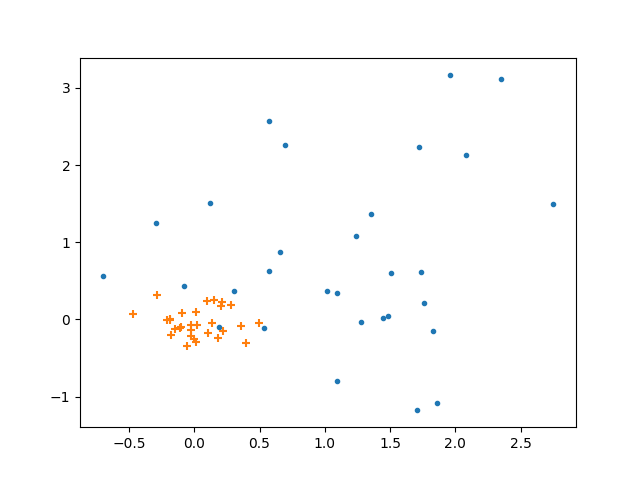
\includegraphics[width=0.6\textwidth]{data.png}
\end{center}

Would the Adaptive RBFN work (i.e. propose a reasonable decision boundary)?  If so, how would the parameters (i.e. bases, weights, and biases) possibly look like?  If not, how can we improve it?  \emph{You don't have to answer with math equations; plain English is fine.}

\vspace{30mm}

\paragraph{5. k-NN classifier with Scikit-learn and RBFN with Stochastic Gradient Descent (20 points each)}


%\bibliographystyle{abbrv}
%\bibliography{../lecture_note}


\end{document}






